\section{Emergent Coordinates via Manifold Reconstruction}
  \label{subsec:emergent-coordinates}

  The coordinate chart $x^\mu$ is not postulated in the relational ontology.
  Instead, when the relational distance matrix $D=\{d_{ij}\}$ admits a low-dimensional
  embedding, the coordinates can be \emph{reconstructed} from $D$ by using standard manifold
  learning techniques.

  \subsection{MDS embedding from relational distances}
  \label{subsec:mds-embedding-from-relational-distances}
  Compute the centered Gram matrix
  \begin{equation}
    G_{ij} \;=\; -\frac{1}{2}\Big(d_{ij}^2 - d_{i\cdot}^2 - d_{\cdot j}^2 + d_{\cdot\cdot}^2\Big),
    \label{eq:gram-matrix}
  \end{equation}
  where $d_{i\cdot}^2=\frac{1}{N}\sum_k d_{ik}^2$ and $d_{\cdot\cdot}^2=\frac{1}{N^2}\sum_{k\ell} d_{k\ell}^2$.
  Diagonalizing $G$ yields the eigenpairs $(\lambda_k, v_k)$.
  The embedding in $\mathbb{R}^d$ is then obtained by
  \begin{equation}
    x_i^{(a)} \;=\; \sqrt{\lambda_a}\, (v_a)_i,
    \qquad a=1,\dots,d,
    \label{eq:mds-embedding}
  \end{equation}
  so that $d_{ij}\approx \|x_i-x_j\|$ in the projectable regime.

  The reconstructed coordinates are defined up to global isometries
  (reflections, translations, and rotations), that carry no physical
  significance at the relational level.

  \subsection{Intrinsic dimension from the eigenvalue gap}
  \label{subsec:intrinsic-dimension-from-the-eigenvalue-gap}
  The embedding dimension $d$ is not assumed but is selected by the dominant eigenvalue
  gap $\Delta\lambda_k=\lambda_k-\lambda_{k+1}$.
  Operationally, choose $d$ is chosen as the smallest integer such that
  \begin{equation}
    \Delta\lambda_{d+1} \;>\; \eta\,\lambda_1,
    \label{eq:eigen-gap-criterion}
  \end{equation}
  with a conservative threshold $\eta\sim 0.1$.
  For smooth large-scale configurations, one expects stable low-dimensional embedding
  (often $d=4$ for spacetime-like regimes).

  The spectral criterion used to identify a robust intrinsic dimension is illustrated
  in Fig.~\ref{fig:eigenvalue-gap}.

  \begin{figure}[t]
    \centering
    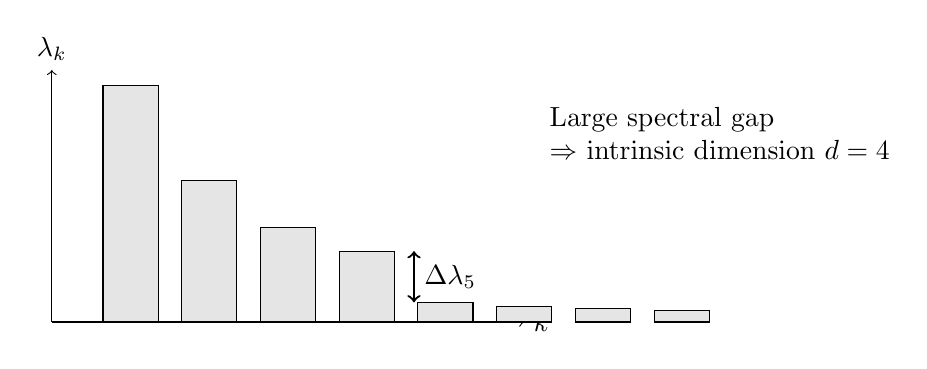
\begin{tikzpicture}[scale=1.0]
        \draw[->] (0,0) -- (6,0) node[right]{$k$};
        \draw[->] (0,0) -- (0,3.2) node[above]{$\lambda_k$};

        % Bars (schematic)
        \foreach \k/\h in {1/3.0,2/1.8,3/1.2,4/0.9,5/0.25,6/0.20,7/0.17,8/0.15} {
          \draw[fill=black!10] (\k-0.35,0) rectangle (\k+0.35,\h);
        }

        % Gap marker
        \draw[<->, thick] (4.6,0.9) -- (4.6,0.25) node[midway,right]{$\Delta\lambda_5$};
        \node[align=left, anchor=west] at (6.2,2.4)
          {Large spectral gap\\$\Rightarrow$ intrinsic dimension $d=4$};
    \end{tikzpicture}
    \caption{\textbf{Schematic eigenvalue spectrum used to select the intrinsic embedding dimension.}
    A clear gap after the first four modes indicates a robust $d=4$ projectable regime.}
    \label{fig:eigenvalue-gap}
  \end{figure}

  \subsection{Breakdown as a physical prediction}
  \label{subsec:breakdown-as-a-physical-prediction}
  The reconstruction may fail when (i) connectivity becomes highly non-local or (ii) the
  spectrum of $G$ exhibits no clear gap (glassy/fractal regimes).
  This behavior should not be interpreted as a pathology of the reconstruction.
  Rather, it signals a transition to a pre-geometric regime in which a smooth
  continuum manifold ceases to provide an adequate effective description.

  \paragraph{From relational structure to geometric representation.}
    At the relational level, the configurations of \(\chi\) are specified entirely by the
    internal structural relations and bounded relaxation constraints.
    No notions of distance, angle, or curvature were defined.
    However, when relational variations become sufficiently smooth and hierarchically
    organized, these configurations can be represented using effective
    geometric descriptors.

    This representation associates relational gradients with spatial gradients of a
    projected field \(\chi_{\mathrm{eff}}\), and collective relaxation constraints with
    geometric quantities such as curvature or gravitational potential.
    The resulting geometric language provides a compact and operationally useful
    summary of relational organization, but it is neither unique nor exact.

  \paragraph{Status of the effective metric.}
    The effective metric introduced in the main text has not yet been postulated as a fundamental object.
    It is defined implicitly through the propagation properties of perturbations and
    an operational comparison of the relaxation rates.
    Thus, the metric encodes how relational distinctions are mapped onto
    effective notions of spatial separation and temporal ordering.

    As this mapping is many-to-one, distinct relational configurations may
    correspond to the same effective metric.
    Conversely, changes in the relational structure may occur without
    corresponding changes in the effective geometric description.
    Therefore, the metric captures only a restricted subset of the information
    contained in the relational configuration.

  \paragraph{Emergence of field equations.}
    The Poisson-type and wave-like equations appearing in the effective description arise
    from linearizing the relational relaxation dynamics around quasi-homogeneous configurations.
    They express how small deviations from the uniform relaxation propagate and combine at the macroscopic level.

    These equations should not be interpreted as fundamental dynamic laws.
    These are regime-dependent approximations whose validity is limited to weak-field, slow-variation conditions.
    Outside these regimes, an effective geometric description ceases to provide a
    faithful account of the underlying relational dynamics.

    Poisson-type and wave-like equations arise by linearizing the
    \emph{projected} relational relaxation dynamics around quasi-homogeneous configurations.

  \paragraph{Consistency across descriptive levels.}
    No contradiction exists between relational and geometric formulations.
    They apply different descriptive levels of the same underlying theory.
    The relational formulation specifies the fundamental ontology and dynamics,
    whereas the geometric description provides an efficient and empirically successful
    approximation in the appropriate regimes.

    Importantly, the direction of conceptual dependence is unambiguous:
    the geometric description depends on the relational one, but not conversely.
    All geometric notions are secondary constructs whose meaning and applicability are
    derived from the relational organization of \(\chi\).

  \paragraph{Conceptual role.}
    This subsection clarifies that the effective geometric language employed throughout
    the main text is a representational tool rather than an ontological commitment.
    Its role is to connect the underlying relational foundations of the framework
    with familiar macroscopic descriptions of spacetime and gravity, while
    preserving the non-geometric nature of the fundamental construction.

    Therefore, the relational formulation underwrites the validity of the effective
    geometric description without being reducible, ensuring conceptual coherence
    across all levels of the framework.

  \input{D-emergent-coordinates/04-example-of-a-robust-spectral-ratio-in-a-relational-laplacian}
